\chapter{System modelling}\label{modelling}
Wireless communication networks have been extensively study in scientific literature and one of the most used mathematical tools to model them and their behaviour is \textit{graph theory}.
In this work the same approach was followed.\\
As the broadcast goes on and the message is transmitted among the nodes, the system goes through different states where each node could be transmitting, listening for an incoming message or could have already sent the message and has stopped.
These different behaviours were modelled by means of three different states:
\begin{itemize}
	\item
	\texttt{listening}: the node has not received the broadcast yet and therefore it is still listening for incoming messages from other nodes.
	\item
	\texttt{transmitting}: the node has received the message and during each slot it is trying to transmit it to adjacent nodes. A node in \texttt{transmitting} state will sometimes be referred as \textit{active} node.
	\item
	\texttt{sleeping}: the node has already received the message and transmitted it in turn. Once a node is in a sleeping state, it has no effect on the system any more.
\end{itemize}


\section{Graph model for wireless systems}

The N users dropped in a floorplan make up the set of vertices V of a graph G, whose set of edges E is composed by all the connections between two nodes in reach of each other. Let us take a simplified scenario to exemplify this approach.
\begin{figure}[h]
	\begin{minipage}{.5\textwidth}
        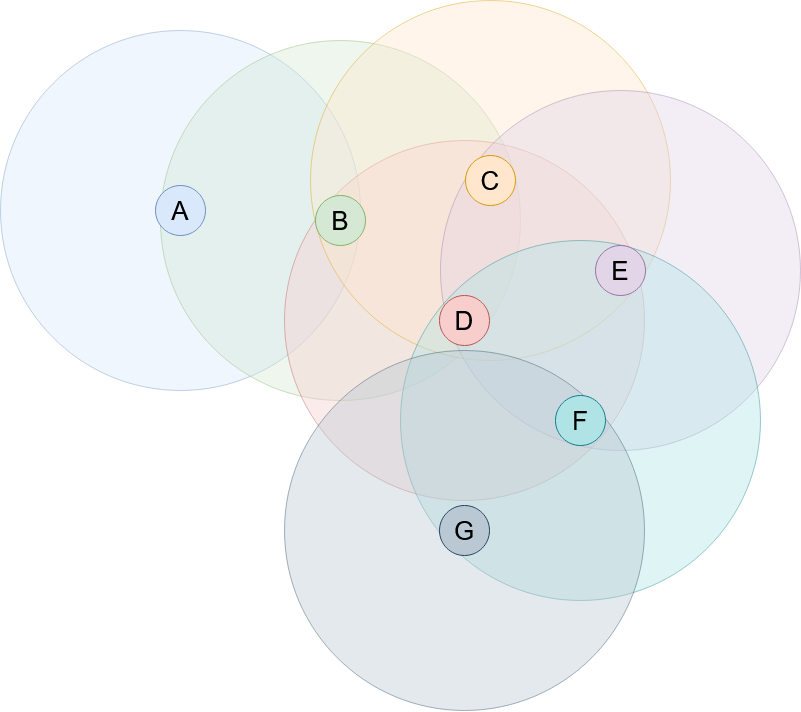
\includegraphics[scale=.23]{img/wireless_graph_1.png}
        \begin{center}
            a) Ranges representation
        \end{center}
	\end{minipage}
	\begin{minipage}{.5\textwidth} 
		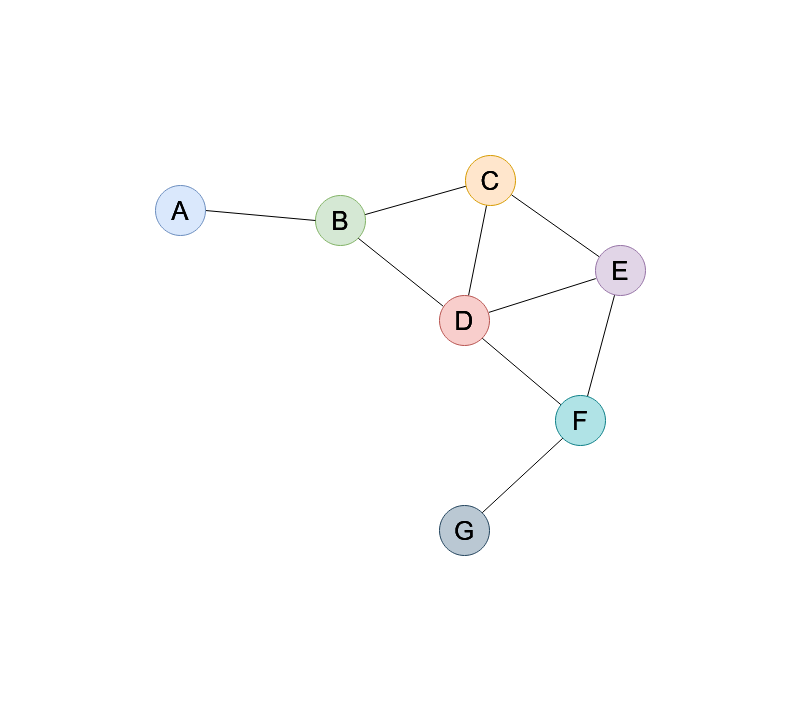
\includegraphics[scale=.23]{img/wireless_graph_2.png}
		\begin{center}
            b) Equivalent graph representation
        \end{center}
	\end{minipage}
	\caption{}
    \label{fig:graph1}
\end{figure}

In Figure \ref{fig:graph1} (a) devices A, C and D are within device B transmission radius. In the equivalent graph, there will be edges that connect B to A, B to C and B to D. The same goes for all the other vertices.\\
In general, the existence of an edge from vertex $i$ to vertex $j$ means that nodes $i$ and $j$ are within reach of each other. Two vertices connected by an edge are said to be \textit{adjacent}. The set of a vertex $v$ together with all its adjacent nodes forms a subgraph called the \textit{neighbourhood of v}.\\
During the broadcast, a node can only receive from and transmit to its neighbourhood.\\
\hfill \break
Once a node has transmitted the message and has gone into \texttt{sleeping} state, it disappears, along with all the edges connected to it. Therefore, the set of vertices V changes with time. This is what in literature is called a \textit{dynamic graph} or, more specifically, a \textit{node-dynamic graph.}

%Should this paragraph be moved to another chapter/section ?
Modelling the system with graphs also allows for the easy computation of a lower bound for the broadcast time \texttt{T}, which can be useful for the validation of the simulator.\\
Given a graph $G(V, E)$ that represents the users in the floorplan, let $v^{*}$ be the starter of the broadcast, i.e. the first node with the message.\\
In a best case scenario, the system evolves with no collisions at all and the message moves along the paths of the graph, reaching all nodes.\\
%TODO add citation to bibliography: [ F. Harary, Graph Theory, Addison-Wesley, 1969, p.199. ]
Let $d(u, v)$ be the \textit{distance} between two vertices $u$ and $v$, i.e. the length of a shortest directed path from u to v consisting of arcs, provided at least one such path exists.\\
Then, the lower bound for the broadcast time is given by the greatest distance between $v^{*}$ and any other vertex. This quantity, in graph theory, is called \textit{eccentricity} of the vertex $v^{*}$. More formally, the eccentricity of $v^{*}$ is defined as follows:

\begin{equation}
\epsilon(v^{*}) = \max_{v{\in}V} d(v^{*}, v)
\end{equation}



\section{Simplified models}

\subsection{Single queue configuration}\label{ssec:singlequeue}

Let us consider a configuration where devices arranged in a line, as shown in Fig. \ref{fig:single_queue}. Each device only has two neighbours, except for the outer ones that only have one. Let assume A to be the broadcast starter. A is in \texttt{transmitting} state while all the other nodes are initially in \texttt{listening} state. 
\hfill \break
\hfill \break

\begin{figure}[H]%
    \centering
	{{
\includegraphics[scale=0.6]{img/single_queue.png} }}%
    \caption{}%
    \label{fig:single_queue}%
\end{figure}

It is clear that, with this configuration, each listening node has a maximum of one active node in its neighbourhood and thus cannot possibly receive the message from two different sources at the same time.
This guarantees the absence of collisions.

In such a scenario, $100\%$ asymptotic coverage is ensured:
during each slot, the active node extracts a Bernoulli RV with success probability $p$. The probability of the active node not transmitting for k consecutive slots is a geometric distribution:

\begin{equation}
	P(X = k) = (1\text{-}p)^{k}
	\label{geometric_distribution}
\end{equation}

The successful transmission of the message from an active node to its neighbour is thus guaranteed since $\lim_{k \to \infty} (1\text{-}p)^{k} = 0$

%TODO not really sure about this result when the starter node is not the first or the last. What if the starter node is in the middle of the queue?
As for the total broadcast time \texttt{T}, on average it is equal to the mean value of the Bernoulli RV, \textit{p}, times the number of hops needed to reach the last node.
%times the eccentricity of the starter, maybe? Not really sure about that, I have to look into it a bit more in detail

\begin{equation}
	E[T] = p \cdot (N-1)
	\label{singleQueueMeanT}
\end{equation}

\subsection{Star configuration with one active node}
Another useful simple configuration worth analysing is a star-shaped configuration. In this setup, there is a central node A connected to N-1 nodes, all of which are non-adjacent to each other. Let us suppose A to be the broadcast starter.

\begin{figure}[H]%
    \centering
	{{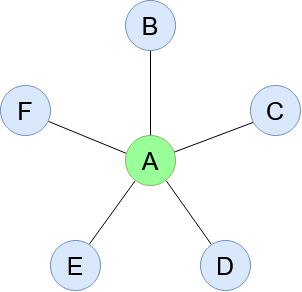
\includegraphics[scale=0.5]{img/star_graph.png} }}%
    \caption{}%
    \label{fig:star_graph}%
\end{figure}

The absence of collisions is ensured in this scenario as well, for the same reason as the previous example.\\
At each slot, A keeps extracting a Bernoulli RV. When the extraction is successful, A broadcasts the message to all its neighbour and total coverage is reached. Hence, 100\% asymptotic coverage is ensured in this case too, as the probability of A not transmitting for k consecutive slots is Eq. \ref{geometric_distribution} and goes to 0 as k goes to infinity.\\
In this case, the average total broadcast time E[\texttt{T}] is simply equal to the mean value of the Bernoulli RV \textit{p}.

If the broadcast starter was one of the ``rays" of the star, instead of the center, there would not be much difference: absence of collisions and total coverage would be ensured as well.\\
As for \texttt{T}, its expected value would just be $2p$, since the are now \textbf{two} hops involved in the broadcast: one from the starter to the center of the star and the other from the center node to all the N-2 remaining ones.

\subsection{Star configuration with all but one active nodes}
\label{ssec:star2}

This configuration can be seen as the complement of the previous one: every ``ray" of the star is active and trying to transmit the message to the center node.

\begin{figure}[H]%
    \centering
	{{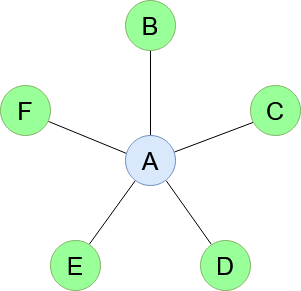
\includegraphics[scale=0.5]{img/star_graph2.png} }}%
    \caption{}%
    \label{fig:star_graph}%
\end{figure}

Now there is the possibility of collisions and a non-zero probability that there will never be total coverage.

To simplify the analysis of this system and obtain some more insight, it is useful to model it by means of a discrete-time Markov chain.

%TODO choose better title for subsection, maybe?
\subsubsection{Discrete-time Markov chain model for N nodes transmitting to a target}
Since the state of the system evolves only once per slot, it can be modelled with a discrete-time Markov chain (DTMC).
\hfill \break
\hfill \break

\begin{figure}[H]%
    \centering
	{{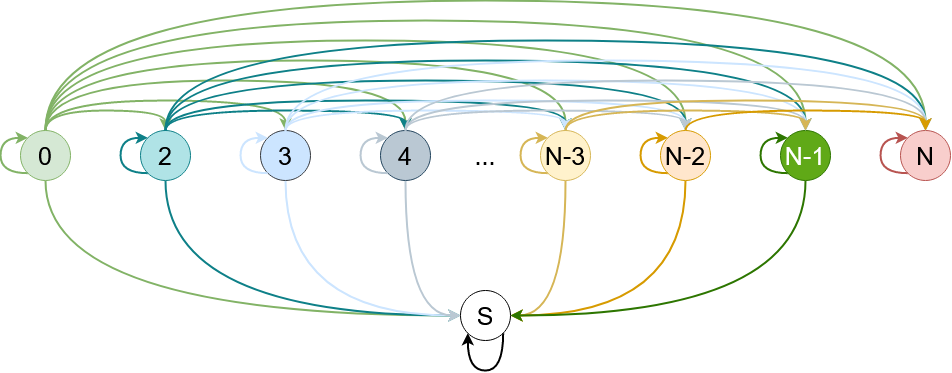
\includegraphics[scale=0.4]{img/DTMC.png} }}%
    \caption{Discrete-time Markov chain for a scenario with N active devices}%
    \label{fig:dtmc}%
\end{figure}

\noindent Figure \ref{fig:dtmc} shows the DTMC for a generic configuration with N transmitters (transition probabilities are not shown for the sake of clarity).\\
State 0 and states 2 to N represent the number of \texttt{sleeping} devices, namely devices that have already sent the message and have stopped. 
State S represents the successful transmission state, which the system transitions to when only one device has transmitted the message during the previous slot.

The initial state $X_{0}$ is 0. Any transition from a state $i$ to a state $j$, $j \neq S$, means that more than one device has transmitted the message and consequently the target device has detected a collision.
Both state S and state N are \textit{absorbing states}, i.e. states that, once entered, cannot be left (as can be seen in Fig. \ref{fig:dtmc}, where the only outgoing arrow from each of the two goes back to the state itself).

If the system transitions to state N, it stays in it indefinitely since all the devices would be \texttt{sleeping} and they cannot become active again. This implies that there will never be total coverage since the target device will forever stay in a \texttt{listening} state.\\
%TODO improve? Is it clear?
On the other hand, state S, although being an absorbing state as well, should actually be considered an ``exit" instead of a ``sink": if the system transitions to it, the target device has successfully received the message and the DTMC does not model the system any more.\\
Another interesting observation concerns state N-1: once the system reaches this state, it would be guaranteed that the target device will sooner or later receive the message, for the same reason set forth in \ref{ssec:singlequeue}.

\subsubsection{Transition probabilities}

Let us now address the challenging part: computing the transition probability.
\hfill \break
During the first slot, the probability that $j$ devices out of $N$ transmit the message is the following:

\begin{equation}
	P_{1}(j, N) = {N\choose j} p^{j} (1-p)^{N-j}
	\label{eq:firstSlotTransProb}
\end{equation}

\noindent Derivation of \ref{eq:firstSlotTransProb} can be found in Appendix A.\\

As for the probability of $j$ devices transmitting at the same time during slot $k$, be it $P_{k}(j)$, we can model the system as if it was in the first slot, with the total number of active devices now being equal to $N$ - $t$, where $t$ is the total number of devices that have transmitted up to the $(k\text{-}1)$-th slot.\\
%TODO fix
The problem with this formulation is... Is what? \\

A better way to compute the probability of having $j$ devices transmitting at slot $k$, is to use the \textit{stochastic matrix} of the Markov chain.

If the probability of moving from state $i$ to $j$ in one time slot is $Pr(j|i) = P_{i,j}$, the stochastic matrix P is given by using $P_{i,j}$ as the i-th row and j-th column element, e.g.

\begin{equation*}
P = 
\begin{bmatrix}
P_{0,0}	& P_{0,S}	& P_{0,2}	& \dots  	& P_{0,j}	& \dots		& P_{0,N} \\
P_{S,0}	& P_{S,S}	& P_{S,2}	& \dots  	& P_{S,j}	& \dots		& P_{S,N} \\
P_{2,0}	& P_{2,S}	& P_{2,2}	& \dots  	& P_{2,j}	& \dots		& P_{2,N} \\
\vdots	& \vdots	& \vdots	& \ddots 	& \vdots	& \ddots	& \vdots \\
P_{i,0}	& P_{i,S}	& P_{i,2}	& \dots		& P_{i,j}	& \dots		& P_{i,N} \\
\vdots	& \vdots	& \vdots	& \ddots	& \vdots	& \ddots	& \vdots \\
P_{N,0}	& P_{N,S}	& P_{N,2}	& \dots		& P_{N,j}	& \dots		& P_{N,N} \\
\end{bmatrix}
\label{stochasticMatrix1}
\end{equation*}
\hfill \break
Since S and N are absorbing states, $P_{S,j}=0$ for j $\neq$ S and $P_{N,j}=0$ for j $\neq$ N.\\
Moreover, all the possible transitions can only generate a non-decreasing sequence of states, hence $P_{i, j} = 0 $ $ \forall i > j $.\\
All the other elements of the matrix can be computed using formula \ref{eq:firstSlotTransProb}:

 \begin{equation}
	P_{i,j} = {N-i\choose j} p^{j} (1-p)^{N-i-j}
	\label{eq:matrixElementProb}
\end{equation}
\hfill \break
Therefore the stochastic matrix becomes:

\begin{equation*}
P = 
\begin{bmatrix}
P_{0,0}	& P_{0,S}	& P_{0,2}	& \dots  	& P_{0,j}	& \dots		& P_{0,N} \\
0		& 1			& 0			& \dots  	& 0			& \dots		& 0		 \\
0		& P_{2,S}	& P_{2,2}	& \dots  	& P_{2,j}	& \dots		& P_{2,N} \\
\vdots	& \vdots	& \vdots	& \ddots 	& \vdots	& \ddots	& \vdots \\
0		& P_{i,S}	& 0			& \dots		& P_{i,j}	& \dots		& P_{i,N} \\
\vdots	& \vdots	& \vdots	& \ddots	& \vdots	& \ddots	& \vdots \\
0		& 0			& 0			& \dots  	& 0			& \dots		& 1		 \\
\end{bmatrix}
\label{stochasticMatrix2}
\end{equation*}
\hfill \break
Let $x_{0}$ be the \textit{initial state vector}, i.e. an $N \times 1$ vector that describes the probability distribution of starting at each of the N possible states.\\
To compute the probability of transitioning to state $j$ in \textbf{k} steps, it is now sufficient to multiply the initial state vector $x_{0}$ by the stochastic matrix raised to the k-th power, e.g.

\begin{equation}\label{probAtStateK1}
P_{k}(j) = x_{0}\cdot P^{k}
\end{equation}
\hfill \break
In our case, the system always starts in state 0, so we have

\begin{equation*}
x_{0} = 
\begin{bmatrix}
1 \\
0 \\
0 \\
\vdots \\
0
\end{bmatrix}
\label{initialStateVector}
\end{equation*}
\hfill \break
which yields

\begin{equation}
P_{k}(j) = 
\begin{bmatrix}
1 \\
0 \\
0 \\
\vdots \\
0
\end{bmatrix}
\cdot P^{k} = (P^{k})_{0,j}
\label{eq:Pk_of_j}
\end{equation}
\hfill \break

Calculating the k-th power of a matrix can be an intensive task from a computational point of view. To improve the complexity of the computation, rows and columns of P can be rearranged, moving the S row and the S column as penultimate, thus obtaining

\begin{equation*}
P = 
\begin{bmatrix}
P_{0,0}	& P_{0,2}	& P_{0,3}  	& \dots	& P_{0, N-1}	& P_{0,S}	& P_{0,N} \\
		& P_{2,2}	& P_{2,3}  	& \dots	& P_{2, N-1}	& P_{2,S}	& P_{2,N} \\
		& 			& P_{3,3}	& \dots	& P_{3, N-1}	& P_{3,S}	& P_{3,N} \\
 		& 			& 			& \ddots& \vdots		& \vdots	& \vdots \\
		& 			& 			& 		& P_{N-1,N-1}	& P_{N-1,S}	& P_{N-1, N}\\
		& 			& 			& 		& 				& 1			& 0		 \\
0		& 			& 		  	& 		& 				& 			& 1		 \\
\end{bmatrix}
\label{triangularPMatrix}
\end{equation*}
\hfill \break

P is now an upper triangular matrix and this allows for faster computation of its powers in \ref{eq:Pk_of_j} .


%TODO add something about the number of collisions maybe?
